%!TEX root = ../main.tex
\begin{figure}[h]
    \centering
    \begin{subfigure}[b]{1\textwidth}
    \centering
    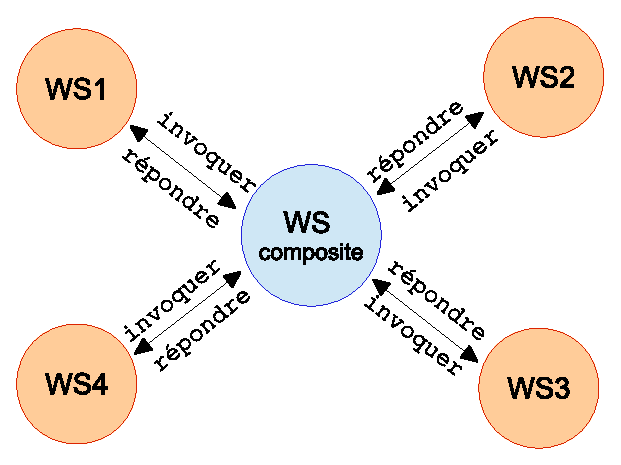
\includegraphics[width=0.7\textwidth]{figs/orchestration.eps}
    \caption{l'orchestration des services.}
    \label{fig:orchestration}
    \end{subfigure}

    \begin{subfigure}[b]{1\textwidth}
    \centering
    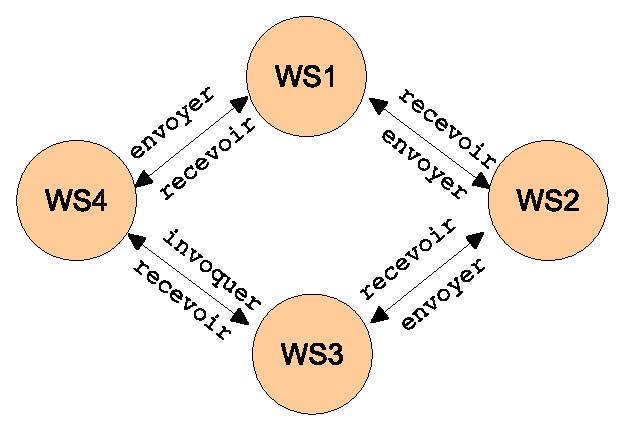
\includegraphics[width=0.7\textwidth]{figs/choregraphie.eps}
    \caption{la chorégraphie des services.}
    \label{fig:choregraphie}
    \end{subfigure}

    \caption{Orchestration vs Chorégraphie.}
    \label{fig:orchestration-vs-choregraphie}
\end{figure}

%%% Local Variables:
%%% mode: latex
%%% TeX-master: "../main"
%%% End: